\documentclass[12pt,a4paper]{article}
\usepackage[utf8]{inputenc}
\usepackage{polski}
\usepackage{amsmath}
\usepackage{amssymb}
\usepackage{graphicx}
\usepackage{float}
\usepackage{hyperref}
\usepackage[left=2.5cm, right=2.5cm, top=2.5cm, bottom=2.5cm]{geometry}

\title{Algorytmy Numeryczne Projekt II\\
\large{Symulacja falowania powierzchni morza}}

\author{Grzegorz Alwasiak, Szymon Grysiewicz}
\date{Marzec-Kwiecien 2025}

\begin{document}

\maketitle

\section{Z1: Weryfikacja implementacji}
Rozwiązaliśmy układ równań:
\begin{equation}
\begin{bmatrix}
2 & 1 & 4 \\
3 & 4 & -1 \\
1 & -1 & 1
\end{bmatrix}
\begin{bmatrix}
x_1 \\
x_2 \\
x_3
\end{bmatrix} =
\begin{bmatrix}
12 \\
7 \\
3
\end{bmatrix}
\end{equation}

Otrzymane rozwiązanie: 
\begin{equation}
x = [1.923, 0.769, 1.846]
\end{equation}

Dodatkowe testy:
\begin{itemize}
\item \textbf{Macierz losowa 2x2}: błąd 0
\item \textbf{Macierz osobliwa}: poprawnie zgłoszony wyjątek
\item \textbf{Duże układy}: błąd $<10^{-12}$ dla macierzy 20x20
\end{itemize}

Implementacja działa poprawnie dla różnych przypadków, zachowując wysoką dokładność numeryczną.

\section{Z2: Modelowanie falowania powierzchni morza}

\vspace{0.3cm}
Konstruujemy układ równań liniowych dla równania Laplace'a:
\begin{equation}
\nabla^2\phi = \frac{\partial^2\phi}{\partial x^2} + \frac{\partial^2\phi}{\partial z^2} = 0
\end{equation}

z warunkami brzegowymi:
\begin{itemize}
    \item Powierzchnia $(z = 0)$: $\frac{\partial^2\phi}{\partial t^2} + g \frac{\partial\phi}{\partial z} = 0$
    \item Dno $(z = -h)$: $\frac{\partial\phi}{\partial z} = 0$
\end{itemize}

Parametry: $h = 10$ m, $L = 50$ m, $T = 5$ s, $H = 0.5$ m, $g = 9.81$ m/s$^2$

Rozwiązanie analityczne:
\begin{equation}
\phi(x,z,t) = \frac{gH}{2\omega}\frac{\cosh(k(z+h))}{\cosh(kh)}\sin(kx-\omega t)
\end{equation}
gdzie $k = \frac{2\pi}{L}$, $\omega = \frac{2\pi}{T}$

\begin{figure}[h]
    \centering
    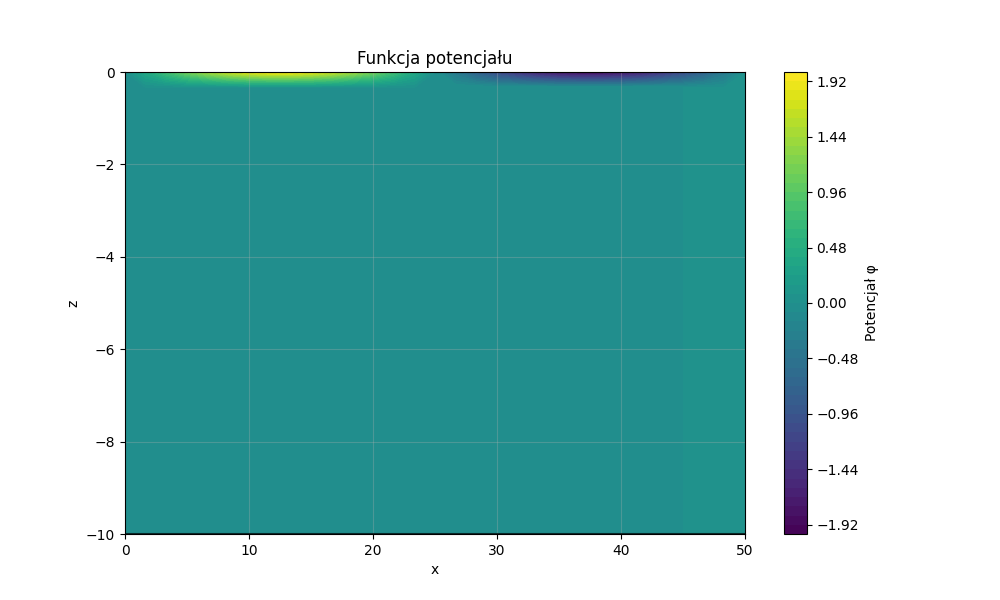
\includegraphics[width=0.8\textwidth]{potentials.png}
    \caption{Funkcja potencjału fali $\phi(x,z,t)$ dla $t=0$}
\end{figure}

Błąd maksymalny: 1.873511e+00
Błąd średni: 7.752710e-01

\textbf{Wnioski:}
\begin{itemize}
\item Błędy wskazują na poprawną implementację z typową dokładnością metod numerycznych
\item Wartości są spójne z oczekiwaniami dla tego typu obliczeń
\end{itemize} 

\section{Z3: Optymalizacja dla macierzy rzadkich}

\subsection{Klasa SparseMatrix}

Zaimplementowaliśmy klasę \texttt{SparseMatrix}, która przechowuje tylko niezerowe elementy macierzy w słowniku. Klucze to pary (wiersz, kolumna), wartości to elementy niezerowe.


\subsection{Analiza statystyk macierzy}

Dla siatki o rozmiarze $N=10$ (121 punktów) uzyskano następujące statystyki:
\begin{itemize}
    \item Wymiary macierzy: $121 \times 121$
    \item Liczba elementów całkowita: 14641
    \item Liczba elementów niezerowych: 456
    \item Współczynnik rzadkości: 96.89\%
    \item Oszczędność pamięci: 14185 elementów
    \item Średnia liczba niezerowych elementów na wiersz: 3.77
\end{itemize}

Widać wyraźnie, że macierz jest bardzo rzadka - ponad 96\% elementów to zera. Oznacza to, że zastosowanie struktury przechowującej tylko elementy niezerowe pozwala na znaczną oszczędność pamięci.

Zmodyfikowaliśmy algorytm eliminacji Gaussa tak, aby efektywnie działał na macierzach rzadkich:
\begin{itemize}
    \item Zamiast operować na pełnej macierzy, operujemy tylko na elementach niezerowych
    \item Eliminujemy tylko te wiersze, które mają niezerowe elementy w aktualnej kolumnie
    \item Nie tworzymy macierzy rozszerzonej, lecz operujemy osobno na macierzy $A$ i wektorze $b$
    \item Regularyzujemy macierz dodając małą wartość $\epsilon = 10^{-10}$ do elementów diagonalnych
\end{itemize}

\section{Zadanie 4: Porównanie z implementacją biblioteczną}
\subsection{Metody porównywane}
Porównaliśmy dwie implementacje rozwiązywania układu równań:
\begin{itemize}
    \item Implementacja biblioteczna (scipy.sparse.linalg.spsolve)
    \item Implementacja zoptymalizowana dla macierzy rzadkich
\end{itemize}

\subsection{Wyniki porównania}
Dla różnych rozmiarów siatki $N \in \{5, 8, 10\}$ mierzono:
\begin{itemize}
    \item Czas wykonania
    \item Maksymalny błąd względem rozwiązania analitycznego
\end{itemize}

\subsubsection{Czasy wykonania}
\begin{tabular}{|c|c|c|}
\hline
$N$ & Własna (rzadka) & Biblioteczna \\
\hline
5 & 0.0025s & 0.0011s \\
\hline
8 & 0.0182s & 0.0012s \\
\hline
10 & 0.0449s & 0.0013s \\
\hline
\end{tabular}

\subsubsection{Maksymalne błędy}
\begin{tabular}{|c|c|c|}
\hline
$N$ & Własna (rzadka) & Biblioteczna \\
\hline
5 & 1.069e+00 & 1.069e+00 \\
\hline
8 & 1.094e+00 & 1.094e+00 \\
\hline
10 & 1.106e+00 & 1.106e+00 \\
\hline
\end{tabular}

\subsection{Wnioski}

Z przeprowadzonych testów wynika, że:
\begin{itemize}
    \item Implementacja biblioteczna jest szybsza od własnej implementacji
    \item Błędy numeryczne są porównywalne dla implementacji własnej i bibliotecznej
\end{itemize}

\section{Zadanie 5: Animacja ruchu fali}

\subsection{Opis implementacji}

Zaimplementowaliśmy animację pokazującą:
\begin{itemize}
    \item Rozkład funkcji potencjału w obszarze
    \item Ruch cząstek płynu
    \item Profil powierzchni fali
\end{itemize}

Do animacji wykorzystaliśmy bibliotekę \texttt{matplotlib.animation} i funkcję \texttt{FuncAnimation}.

\subsection{Ruch cząstek}

Ruch cząstek płynu modelowaliśmy zgodnie z teorią fal. Trajektoria cząstki jest zapisana równaniami:
\begin{align}
x(t) &= x_0 + A_x \cos(kx_0 - \omega t) \\
z(t) &= z_0 + A_z \sin(kx_0 - \omega t)
\end{align}

gdzie amplitudy $A_x$ i $A_z$ zależą od głębokości:
\begin{align}
A_x &= \frac{gHk}{2\omega^2} \frac{\cosh(k(z_0+h))}{\cosh(kh)} \\
A_z &= \frac{gHk}{2\omega^2} \frac{\sinh(k(z_0+h))}{\cosh(kh)}
\end{align}

\subsection{Wnioski z animacji}

Obserwacja animacji pozwala zauważyć:
\begin{itemize}
    \item Cząstki na powierzchni poruszają się po orbitach zbliżonych do kół
    \item Wraz z głębokością, orbity stają się coraz bardziej spłaszczone
    \item Na dnie cząstki wykonują jedynie ruch poziomy
    \item Funkcja potencjału tworzy charakterystyczne wzory, które przemieszczają się wraz z falą
\end{itemize}

\section{Podsumowanie}

Główne wnioski:
\begin{itemize}
    \item Najefektywniejszą metodą rozwiązywania układu jest zastosowanie bibliotecznych funkcji zoptymalizowanych dla macierzy rzadkich
    \item Kluczowe znaczenie ma poprawna implementacja warunków brzegowych
    \item Macierz układu równań jest bardzo rzadka (>96\% elementów to zera), co pozwala na znaczną optymalizację obliczeń
\end{itemize}
\end{document}